\documentclass[a4paper, 10pt]{article}

\usepackage[english]{babel}
\usepackage[T1]{fontenc}
\usepackage[utf8]{inputenc}
\usepackage{textcomp}
\setlength{\marginparwidth}{2cm}

\usepackage{comment}
\usepackage{todonotes}

\usepackage{amsmath}
\usepackage{amssymb}
\usepackage{latexsym}
\usepackage{bm}

\usepackage{enumitem}
\usepackage{array}
\setlength\extrarowheight{5pt}

\usepackage{xcolor}
\usepackage{graphicx}
\graphicspath{ {./img/} }

\newcommand\scalemath[2]{\scalebox{#1}{\mbox{\ensuremath{\displaystyle #2}}}}

\usepackage{hyperref}
\usepackage{listings}
\usepackage{color}
\definecolor{dkgreen}{rgb}{0,0.6,0}
\definecolor{gray}{rgb}{0.5,0.5,0.5}
\definecolor{mauve}{rgb}{0.58,0,0.82}
\lstset{frame=tb,
    language=Python,
    aboveskip=3mm,
    belowskip=3mm,
    showstringspaces=false,
    columns=flexible,
    basicstyle={\small\ttfamily},
    numbers=none,
    numberstyle=\tiny\color{gray},
    keywordstyle=\color{blue},
    commentstyle=\color{dkgreen},
    stringstyle=\color{mauve},
    breaklines=true,
    breakatwhitespace=true,
    tabsize=3
}

\title{Homework Assignment N°6}
\author{BML36\\Thibault Douzon\\Rajavarman Mathivanan}
\date{October 26th, 2018}

\begin{document}
\maketitle

\pagebreak

\tableofcontents

\pagebreak
\section{Exercise 1: Constrained Optimization}
\subsection{Part a}
We want to minimize $f(x_1,x_2)= x_1^2+3x_2^2-2x_2$ under the constraint $g(x_1,x_2)=x_1+3x_2+2=0$.
\\
The Lagrangian function is given by $L(x_1,x_2,\lambda) = f(x_1,x_2)+\lambda g(x_1,x_2)$
$$
L(x_1,x_2,\lambda) = x_1^2+3x_2^2-2x_2 + \lambda (x_1+3x_2+2)
$$
To minimize $f$, we must solve the set of equations that we obtain when computing the gradient of $L$.
$$
\nabla L(x_1,x_2,\lambda) = 0
$$
$$
\nabla L(x_1,x_2,\lambda) = \left\{ \begin{array}{c}
    2x_1+\lambda = 0\\
    6x_2-2+3\lambda = 0\\
    x_1+3x_2+2=0
\end{array}\right. 
$$
We have 3 unknowns and 3 equations, we should be able to solve it. We can rewrite it under matrix notation:
$$
\begin{bmatrix}
    2 & 0 & 1\\
    0 & 6 & 3\\
    1 & 3 & 0
\end{bmatrix} \cdot \begin{bmatrix}
    x_1\\
    x_2\\
    \lambda
\end{bmatrix} = \begin{bmatrix}
    0\\
    2\\
    -2
\end{bmatrix}
$$
$$
\begin{bmatrix}
    x_1\\
    x_2\\
    \lambda
\end{bmatrix} =\begin{bmatrix}
    2 & 0 & 1\\
    0 & 6 & 3\\
    1 & 3 & 0
\end{bmatrix}^{\!-1} \cdot \begin{bmatrix}
    0\\
    2\\
    -2
\end{bmatrix}
$$
Which is equivalent to the following:
$$
\begin{bmatrix}
    x_1\\
    x_2\\
    \lambda
\end{bmatrix} =\begin{bmatrix}
    3/4 & -1/8 & 1/4\\
    -1/8 & 1/24 & 1/4\\
    1/4 & 1/4 & -1/2
\end{bmatrix} \cdot \begin{bmatrix}
    0\\
    2\\
    -2
\end{bmatrix}
$$
$$
\begin{bmatrix}
    x_1\\
    x_2\\
    \lambda
\end{bmatrix} = \begin{bmatrix}
    -3/4\\
    -5/12\\
    3/2
\end{bmatrix}
$$
Hence the solution of this optimization problem is $(x_1^*,x_2^*)=(-3/4, -5/12)$.\\
We can check that the constraint is verified:
$$
g(x_1^*,x_2^*) = -3/4+3\times (-5/12)+2 =-3/4-5/4+2 = -8/4+2 = 0 
$$
Indeed our solution point respects the constraint. Because $\lambda$ is superior to $0$,
without computing the constraint we could know the constraint was active.
\\
The value of the function we minimized at this point is:
$$
f(x_1^*,x_2^*) = (-3/4)^2+3(5/12)^2-2\times5/12 = 23/12
$$

\subsection{Part b}
In this part we minimize $f$ again but we slightly modify the constraint and add another one.
The first constraint use the previous function $g$: $g(x_1,x_2)\geq 0$\\
The second one uses a function $h(x_1,x_2)=-2x_1+2x_2+1$ and states $h(x_1,x_2)\leq0$
\\
To simplify our resolution, we change to sign of $h$ and also the symbol of inequation. This is
strictly equivalent. We call $\bar{h}(x_1,x_2) = -h(x_1,x_2)$.
\\
Now the second constraint can be written like this: $\bar{h}(x_1,x_2)\geq0$.
\\
Because we now have two constraints, we introduce two unknowns $\lambda$ and $\mu$:
$$
L(x_1,x_2,\lambda,\mu) = f(x_1,x_2)+\lambda g(x_1,x_2)+\mu \bar{h}(x_1,x_2)
$$
$$
L(x_1,x_2,\lambda,\mu) = x_1^2+3x_2^2-2x_2 + \lambda (x_1+3x_2+2) + \mu(2x_1-2x_2-1)
$$
Now we compute its gradient:
$$
\nabla L(x_1,x_2,\lambda,\mu) = \left\{ \begin{array}{c}
    2x_1+\lambda+2\mu\\
    6x_2-2+3\lambda-2\mu\\
    x_1+3x_2+2\\
    2x_1-2x_2-1
\end{array}\right .
$$
According to the Karush-Kuhn-Tucker theorem, the solution is obtained when we have the following:
$$
\left\{ \begin{array}{c}
    \frac{\partial L}{\partial x_1}(x_1,x_2) = 0\\
    \frac{\partial L}{\partial x_2}(x_1,x_2) = 0\\
    g(x_1,x_2) \geq 0\\
    \lambda \leq 0\\
    \lambda g(x_1,x_2) = 0\\
    \bar{h}(x_1,x_2) \geq 0\\
    \mu \leq 0\\
    \mu \bar{h}(x_1,x_2) = 0
\end{array}\right.
$$
Because we want to minimize $f$, $\lambda$ and $\mu$ must be negative or null.
\\
Which translate to the following set of inequations and equations:
$$
\left\{ \begin{array}{c}
    2x_1+\lambda+2\mu = 0\ (1)\\
    6x_2+3\lambda-2\mu -2=0\ (2)\\
    x_1+3x_2+2 \geq 0\\
    \lambda \leq 0\\
    \lambda (x_1+3x_2+2) = 0\ (3)\\
    2x_1-2x_2-1 \geq 0\\
    \mu \leq 0\\
    \mu(2x_1-2x_2-1) = 0\ (4)
\end{array}\right.
$$
Now we need to explore all cases:
\\
\paragraph{If $\lambda=0$}
Let's suppose $\lambda=0$:
\\
Using first equation, we deduce that $x_1=-\mu$. Using the second equation we deduce that $x_2=\mu/3+1/3$
\\
Replace those two values in le fourth equation:
$$
\mu(2(-\mu)-2(\mu/3+1/3)-1) = 0
$$
And simplify:
$$
\mu(-\frac{8}{3}\mu-\frac{5}{3})=0
$$
Hence either $\mu=0$ or $\mu=-5/8$. Both are valid values for $\mu$, we will now assume
$\mu=0$
\\
If $\lambda=\mu=0$, we obtain from the two first equations: $(x_1,x_2) = (0,1/3)$. Those values are the only
posible that satisfy equations (1) and (2) but violate the second constraint:
$$
2x_1-2x_2-1 = -2/3-1 = -5/3 \leq 0
$$
Thus our assumption $\mu=0$ isn't valid.
\\
Let's now assume $\mu=-5/8$
\\
From equations (1) and (2) we deduce the values of a candidate: 
$$
(x_1,x_2) = (-\mu, \frac{2+2\mu}{6})
$$
$$
(x_1,x_2) = (5/8, 1/8)
$$
We can check the constraints:
$$
g(5/8,1/8) = 3 \geq 0
$$
$$
\bar{h}(5/8,1/8) = 0 \geq 0
$$
Thus the point $(5/8, 1/8)$ respects every contraints and is a candidate to the minimum.

\paragraph{If $\mu=0$}
Let's now suppose $\mu=0$ whithout any assumption on $\lambda$:
\\
We deduce from (1) and (2) that $x_1=-\lambda/2$ and $x_2=1/3-\lambda/2$.
\\
We can now replace those values in the third equation:
$$
\lambda((-\lambda/2)+3(1/3-\lambda/2)+2) = 0
$$
And simplify:
$$
\lambda(-2\lambda+3) = 0
$$
The solutions of this equation are $\lambda=0$ and $\lambda=3/2$. But because of our previous work,
we can reject $\lambda=0$ as we already explored this possibility before. We can also reject $\lambda=3/2$ 
as it does not respect the constraint on the langragian multipliers.

\paragraph{If $\lambda\ne0$ and $\mu\ne0$}
This is the last possible case: both $\lambda$ and $\mu$ are non zero.
\\
From equation (3) and (4) we deduce the following system of equations:
$$
\left\{\begin{array}{c}
    x_1+3x_2+2=0\\
    2x_1-2x_2-1=0
\end{array}\right.
$$
Which solutions are given by Cramer's rules:
$$
(x_1,x_2) = \left(\frac{(-2)\times(-2)-1\times3}{1\times(-2)-2\times3}, \frac{1\times1-2\times(-2)}{1\times(-2)-2\times3}\right)
$$
$$
(x_1,x_2) = (-\frac{1}{8}, -\frac{5}{8})
$$
We must now use equations (1) and (2) to compute the Lagrangian multipliers and verify they are rightfully positive:
$$
\left\{\begin{array}{c}
    \lambda+2\mu +2x_1= 0\\
    3\lambda-2\mu -2+6x_2=0\\
\end{array}\right.
$$
$$
\left\{\begin{array}{c}
    \lambda+2\mu -1/4= 0\\
    3\lambda-2\mu -23/4=0\\
\end{array}\right.
$$
Again, Cramer's rule gives us the following solution for $\lambda$ and $\mu$: 
$$
(\lambda,\mu) = \left(\frac{1/4\times(-2)-23/4\times2}{1\times(-2)-3\times2},\frac{1\times23/4-3\times1/4}{1\times(-2)-3\times2}\right)
$$
$$
(\lambda,\mu) = (\frac{12}{8},-\frac{5}{8})
$$
But because the value of $\lambda$ is strictly positive, this point is not a valid candidate for the minimum.

Finally, we found only one candidate for the minimum:
$$
(x_1^*,x_2^*)=(5/8, 1/8)
$$
This is the unique solution of this minimization problem. Constraints are active if and only if
the corresponding langragian multiplier is non zero. 
\\
In our case, $(\lambda, \mu) = (3,0)$, thus only the second constraint is active. That means the point
$(x_1^*,x_2^*)$ lays on the surface described by the second constraint.
\\
The value of the function for this point is:
$$
f(x_1^*,x_2^*) = (5/8)^2 +3(1/8)^2-2\times1/8 = 3/16
$$

\section{Exercise 2: Probabilistic Classification}
\subsection{Part a}
An unbiased estimator of the mean $\bar{x}_n$ is the following:
$$
\bar{x}_N = \frac{1}{N} \sum_{i=1}^N x_i
$$
The base formula for the covariance between two random variables $X$ and $Y$ is the following:
$$
s(X,Y) = \frac{1}{N} \sum_{i=1}^N\sum_{j=1}^N(x_i-E[X])(y_i-E[Y])
$$
But this estimator of the covariance is biased, the forllowing formula corrects this bias:
$$
s^\prime(X,Y) = \frac{1}{N-1} \sum_{i=1}^N\sum_{j=1}^N(x_i-E[X])(y_i-E[Y])
$$
From now on, when talking about covariance, we will use this unbiased formula.
\\
When we apply those formulas to the data, we obtain the following results:
\\
Estimation of $E[A]$:
$$
\bar{a}_N = (1.972, 0.990)
$$
Estimation of $\text{cov}(A)$:
$$
s_A^\prime = \begin{bmatrix}
    2.269 & 0.556\\
    0.556 & 2.591
\end{bmatrix}
$$
Estimation of $E[B]$:
$$
\bar{b}_N = (-2.094, -1.131)
$$
Estimation of $\text{cov}(B)$:
$$
s_B^\prime = \begin{bmatrix}
    2.005 & 0.641\\
    0.641 & 3.117
\end{bmatrix}
$$
\subsection{Part b}
We would like to predict the class of a new point $\bm{x} = (2,1)$ given that
1 and B are normally distributed. First, we can notice that $\bm{x}$ is very close 
to the mean of A: $\bar{a}_N = (1.972, 0.990)$. A first guess could be A, with a high probability.
\\
We are now going to compute the probabilistic classification of $\bm{x}$. To do so, we will
use Baye's equation to compute the posterior using the likelihood, the prior and the evidence:
$$
p(C\vert x) = \frac{p(x \vert C)p(C)}{p(x)}
$$
Because we assumed A and B are normally distributed, we have the following formula to compute the prior:
$$
p(x\vert C) = \frac{1}{(2\pi)^{d/2}\vert\Sigma\vert^{1/2}}e^{-\frac{1}{2}(x-\mu)^\top\Sigma^{-1}(x-\mu)}
$$
Where $X\leadsto \mathcal{N}(\mu,\Sigma)$
\\
The prior is simply the proportion of class C in the database:
$$
p(C) = \frac{\vert C\vert}{\sum_{I\in \text{Classes}} \vert I\vert} = \frac{\vert C\vert}{N}
$$
Where $N$ is the total number of points in the database.
\\
Finally, the evidence is computed based on the likelihood and prior of each classes:
$$
p(x) = \sum_{I\in \text{Classes}} p(x\vert I)p(I)
$$
Here are our results:
\begin{center}
\begin{tabular}{ |c|c|c|c| }
    \hline
    \  & Prior & Likelihood & Prior $\times$ Likelihood \\
    \hline
    A & $3/5$ & $0.067426$ & $0.040456$\\
    \hline
    B & $2/5$ & $0.000897$ & $0.000359$\\
    \hline
\end{tabular}
\end{center}
And the evidence is approximately:
$$
p(x) =  \sum_{I\in \text{Classes}} p(x\vert I)p(I) \approx 3/5\times 0.067426 + 2/5\times 0.000897 \approx 0.040814
$$
Now we can compute the posterior of each class:
\begin{center}
\begin{tabular}{ |c|c| }
    \hline
    \  & Posterior \\
    \hline
    A & $\frac{3/5\times0.067426}{0.040814}\approx0.991$\\
    \hline
    B & $\frac{2/5\times0.000897}{0.040814}\approx0.009$\\
    \hline
\end{tabular}
\end{center}
Hence since $p(A\vert x) > p(B\vert x)$, the probabilistic model predicts $\bm{x}$ is of class A.
\subsection{Part c}
To obtain a ROC curve, we need to introduce another variable, a threshold. We will use
$\theta$ such that $0 \leq \theta \leq 1$. And we will change our prediction algorithm: previously
we chose the class with greatest probability. Our new algorithm will be the following one:
\\
Compute $p(B\vert x)$ the probability of B knowing $x$. We choose to focus on B because B is the positive class. 
If $p(B\vert x) \geq \theta$ then predict B, otherwise
predict A. We notice that with $\theta = 0.5$, this algorithm is the same as the previous one.
\\
Now we discretize the interval $[0;1]$ and let $\theta$ take all those values. For each $\theta$ we 
compute the confusion matrix, TP\textsubscript{rate} and FP\textsubscript{rate}.
\\
TP\textsubscript{rate} and FP\textsubscript{rate} are stored at each step and will be used as coordinates
of point for the ROC curve. This is the ROC curve we obtain:
\\
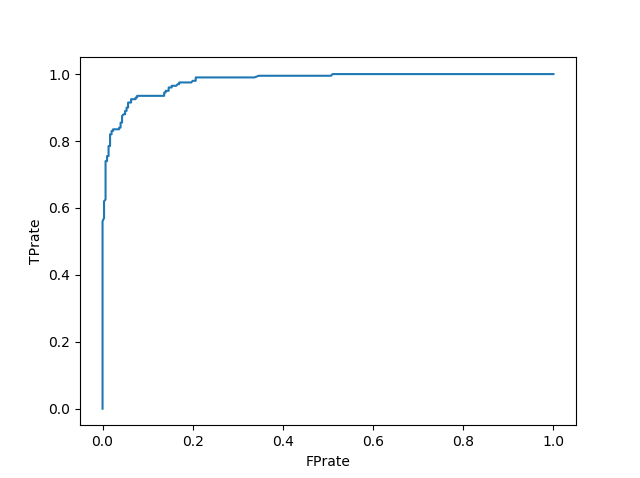
\includegraphics[scale=0.8]{ex2_roc}
\\
What we mean by TP\textsubscript{rate} and FP\textsubscript{rate} are those quantities:
$$
\text{TP}_\text{rate} = \frac{\text{TP}}{\text{TP}+\text{FN}}
$$
$$
\text{FP}_\text{rate} = \frac{\text{FP}}{\text{FP}+\text{TN}}
$$
Our ROC curve shows that the probabilistic model is clearly better than a random model.
The area under the curve is approximately $0.98$ which is excellent.

\section{Exercise 3: PCA}
\subsection{Part a}
We will use the same formula as in the previous exercise for the covariance. The resulting
covariance matrix is the following:
$$
s^\prime_A \approx \begin{bmatrix}
    2.268 & 0.556 & 5.093 \\
    0.556 & 2.591 & 3.703 \\
    5.093 & 3.703 & 13.890
\end{bmatrix}
$$
We can compute its determinant using the maximum precision of the computer:
$$
\vert s^\prime_A\vert \approx 1.913 \cdot 10^{-14} 
$$
Which is so close to $0$ and the precision of the machine, it must be $0$.
\\
This means we can't invert the covariance matrix, and thus because $\Sigma^{-1}$ appears in the formula
of $p(x\vert A)$ we can't either compute the likelihood of $x$.

\subsection{Part b}
To compute the Principal Components of the whole dataset, we first need to compute its covariance matrix.
Let's call $X=A\cup B$, and $\Sigma_X$ its covariance matrix.
$$
\Sigma_X \approx \begin{bmatrix}
    6.134 & 2.662 & 13.445\\
    2.662 & 3.876 & 9.697\\
    13.445 & 9.697 & 35.866
\end{bmatrix}
$$
Now we use Singular Value Decomposition to compute the eigen values and their corresponding eigen vectors of th covariance
matrix.
\\
We obtain the following vector $V$ of eigen values, and matrix $U$ of eigen vectors:
$$
V = [43.569,\ 0.163,\ 2.145]
$$
$$
U = \begin{bmatrix}
    -0.343 & -0.669 & 0.658\\
    -0.244 & -0.613 & -0.750\\
    -0.906 & 0.418 & -0.046
\end{bmatrix}
$$
The Principal Component is simply the direction given by the eigen vector associated
with the largest absolute eigen value.
\\
In our case, the largest eigen value is $43.569$. Hence the principal component is given by the following vector: $\Delta = [-0.343,\ -0.244,\ -0.906]$.
\\
We can now compute the projection of $x$ on the Principal Component:
$$
\text{proj}_\Delta(x) = x_1 = \Delta \cdot x = [-0.343,\ -0.244,\ -0.906] \cdot [1,\ 2,\ 1] \approx -1.739
$$
By doing the projection, we also reduce the number of dimensions of our data. If we only project on the
first Principal Component, the resulting data is 1 dimensional, ie a number.

\subsection{Part c}
To compute the projection of $A$ and $B$ on the first principal component, we apply the same operations to
each point in $A$ and $B$:
$$
\text{proj}_\Delta(x) = x_1 = \Delta \cdot x 
$$
We can now compute mean and covariance on each new dataset, namely $A_1$ and $B_1$:
\begin{center}
\begin{tabular}{ |c|c|c|c| }
    \hline
    \  & Mean & Covariance \\ 
    \hline
    $A_1$ & $-5.392$ & $16.752$ \\
    \hline
    $B_1$ & $4.946$ & $19.637$ \\
    \hline
\end{tabular}
\end{center}
Because $A_1$ and $B_1$ are both 1-dimensional, the covariance matrix is actually a single number: the variance.
\subsection{Part d}
If we assume $A_1$ and $B_1$ are also normally distributed, we can easily compute the likelihood of 
$x_1$ using the normal distribution formula:
\\
If $C\leadsto\mathcal{N}(\mu, \Sigma)$, then:
$$
p(x\vert C) = \frac{1}{(2\pi)^{d/2}\vert\Sigma\vert^{1/2}}e^{-\frac{1}{2}(x-\mu)^\top\Sigma^{-1}(x-\mu)}
$$
Which simplifies in case of a 1-dimensional data:
$$
p(x\vert C) = \frac{1}{(2\pi\Sigma)^{1/2}}e^{-\frac{1}{2}(x-\mu)^2\Sigma^{-1}}
$$
In our case, we get the following:
$$
p(x_1\vert A_1) = \frac{1}{(2\pi\Sigma_{A_1})^{1/2}}e^{-\frac{1}{2}(x_1-\mu_{A_1})^2\Sigma_{A_1}^{-1}}
$$
$$
p(x_1\vert A_1) \approx \frac{1}{(2\pi\cdot16.752)^{1/2}}e^{-\frac{1}{2}((-1.739)-(-5.392))^216.752^{-1}}
$$
$$
p(x_1\vert A_1) \approx 0.065449
$$
And for $B_1$:
$$
p(x_1\vert B_1) = \frac{1}{(2\pi\Sigma_{B_1})^{1/2}}e^{-\frac{1}{2}(x_1-\mu_{B_1})^2\Sigma_{B_1}^{-1}}
$$
$$
p(x_1\vert B_1) \approx \frac{1}{(2\pi\cdot19.637)^{1/2}}e^{-\frac{1}{2}((-1.739)-(4.946))^219.637^{-1}}
$$
$$
p(x_1\vert B_1) \approx 0.028853
$$
We will use the same model as in exercise 1: compute the prior for each class, the evidence and finally the posterior for $A_1$ and $B_1$.
\\
Here are our results:
\begin{center}
\begin{tabular}{ |c|c|c| }
    \hline
    \  & Prior & Likelihood \\
    \hline
    $A_1$ & $3/5$ & $0.065449$ \\
    \hline
    $B_1$ & $2/5$ & $0.028853$ \\
    \hline
\end{tabular}
\end{center}
$A_1$nd the evidence is approximately:
$$
p(x) =  \sum_{I\in \text{Classes}} p(x\vert I)p(I) \approx 3/5\times 0.065449 + 2/5\times 0.028853 \approx 0.050811
$$
Now we can compute the posterior of each class:
\begin{center}
\begin{tabular}{ |c|c| }
    \hline
    \  & Posterior \\
    \hline
    $A_1$ & $\frac{3/5\times0.065449}{0.050811}\approx0.773$\\
    \hline
    $B_1$ & $\frac{2/5\times0.028853}{0.050811}\approx0.227$\\
    \hline
\end{tabular}
\end{center}
Hence since $p(A_1\vert x_1) > p(B_1\vert x_1)$, the probabilistic model predicts $x_1$ is of class $A_1$.
\\
That means that $x$ is classified as $A$ by our model.

\section{Exercise 4: Breast Cancer Case}
In the whole exercise, the prior for benign sample is $0.655$ and for malignant is $0.345$.
\subsection{Part a}
\paragraph{Uniformity of cell shape only}
In this part we will only work with the fourth feature called «Uniformity of cell shape».
If we assume the data along this feature is normally distributed for each class, we can compute
estimators for the Gaussian distributions using the formulas from exercise 2:
\begin{center}
    \begin{tabular}{ |c|c|c| }
        \hline
        \ & Mean & Variance \\
        \hline
        Benign & $1.398$ & $ 0.927$ \\
        \hline
        Malignant & $6.741$ & $6.630$ \\ 
        \hline
    \end{tabular}
\end{center}
We can now use a bayesian model to predict if a tumor is benign or malignant knowing its «uniformity».
\\
We obtain the following confusion matrix on learning data:
\begin{center}
    \begin{tabular}{ |c|c|c| }
        \hline
        Prediction $\backslash$ Reality & Benign & Malignant \\
        \hline
        Benign & $254$ & $16$ \\
        \hline
        Malignant & $12$ & $127$ \\ 
        \hline
    \end{tabular}
\end{center}
Which means a precision of $0.914$ for the malignant tumors and a recall of $0.888$.
\\
We can also use our model on the validation dataset:
\begin{center}
    \begin{tabular}{ |c|c|c| }
        \hline
        Prediction $\backslash$ Reality & Benign & Malignant \\
        \hline
        Benign & $171$ & $16$ \\
        \hline
        Malignant & $7$ & $80$ \\ 
        \hline
    \end{tabular}
\end{center}
Which means a precision of $0.920$ for the malignant tumors and a recall of $0.833$ which is similar to
the results we had on the training set.

\paragraph{First principal component}
In this part we will only work with the first principal component. We compute it by calculating the
eigenvectors of the covariance matrix. The eigenvector related to the largest eigenvalue is the following:
$$
\begin{bmatrix}
    -0.290\\
    -0.406\\
    -0.401\\
    -0.342\\
    -0.236\\
    -0.445\\
    -0.293\\
    -0.342\\
    -0.115
\end{bmatrix}
$$
If we assume the projected data along this direction is normally distributed for each class, we can compute
estimators for the Gaussian distributions using the formulas from exercise 2:
\begin{center}
    \begin{tabular}{ |c|c|c| }
        \hline
        \ & Mean & Variance \\
        \hline
        Benign & $-4.682$ & $3.378$ \\
        \hline
        Malignant & $-18.157$ & $18.249$ \\ 
        \hline
    \end{tabular}
\end{center}
We can now use a bayesian model to predict if a tumor is benign or malignant knowing its position in our high dimensional space.
\\
We obtain the following confusion matrix on learning data:
\begin{center}
    \begin{tabular}{ |c|c|c| }
        \hline
        Prediction $\backslash$ Reality & Benign & Malignant \\
        \hline
        Benign & $258$ & $4$ \\
        \hline
        Malignant & $8$ & $139$ \\ 
        \hline
    \end{tabular}
\end{center}
Which means a precision of $0.946$ for the malignant tumors and a recall of $0.972$.
\\
We can also use our model on the validation dataset:
\begin{center}
    \begin{tabular}{ |c|c|c| }
        \hline
        Prediction $\backslash$ Reality & Benign & Malignant \\
        \hline
        Benign & $173$ & $2$ \\
        \hline
        Malignant & $5$ & $94$ \\ 
        \hline
    \end{tabular}
\end{center}
Which means a precision of $0.949$ for the malignant tumors and a recall of $0.979$ which is similar to
the results we had on the training set.

\paragraph{Uniformity of cell shape and Mitoses}
In this part we will work with the fourth and the ninth features.
If we assume the data along these features is normally distributed for each class, we can compute
estimators for the Gaussian distributions using the formulas from exercise 2:
\begin{center}
    \begin{tabular}{ |c|c|c| }
        \hline
        \ & Mean & Covariance \\
        \hline
        Benign & $\begin{bmatrix}
            1.398 & 1.067
        \end{bmatrix}$ & $\begin{bmatrix}
            9.273\cdot10^{-01} & -6.525\cdot10^{-04}\\
            -6.525\cdot10^{-04} & 2.293\cdot10^{-01}
        \end{bmatrix}$ \\
        \hline
        Malignant & $\begin{bmatrix}
            6.741 & 2.503
        \end{bmatrix}$ & $\begin{bmatrix}
            6.629 & 1.560\\
            1.560 & 6.181
        \end{bmatrix}$ \\ 
        \hline
    \end{tabular}
\end{center}
We can now use a bayesian model to predict if a tumor is benign or malignant knowing its «uniformity» and its «mitoses».
\\
We obtain the following confusion matrix on learning data:
\begin{center}
    \begin{tabular}{ |c|c|c| }
        \hline
        Prediction $\backslash$ Reality & Benign & Malignant \\
        \hline
        Benign & $259$ & $25$ \\
        \hline
        Malignant & $7$ & $118$ \\ 
        \hline
    \end{tabular}
\end{center}
Which means a precision of $0.944$ for the malignant tumors and a recall of $0.825$.
\\
We can also use our model on the validation dataset:
\begin{center}
    \begin{tabular}{ |c|c|c| }
        \hline
        Prediction $\backslash$ Reality & Benign & Malignant \\
        \hline
        Benign & $172$ & $18$ \\
        \hline
        Malignant & $6$ & $78$ \\ 
        \hline
    \end{tabular}
\end{center}
Which means a precision of $0.929$ for the malignant tumors and a recall of $0.813$ which is similar to
the results we had on the training set.

\paragraph{Two firsts principal components}
In this part we will work with the two firsts principal components. We compute it by calculating the
eigenvectors of the covariance matrix. The eigenvectors related to the two largest eigenvalues are the following:
$$
\begin{bmatrix}
    -0.290\\
    -0.406\\
    -0.401\\
    -0.342\\
    -0.236\\
    -0.445\\
    -0.293\\
    -0.342\\
    -0.115
\end{bmatrix}\text{ and } \begin{bmatrix}
    0.125\\
   -0.245\\
   -0.184\\
    0.117\\
   -0.213\\
    0.759\\
   -0.031\\
   -0.469\\
   -0.177
\end{bmatrix}
$$
If we assume the data along these directions is normally distributed for each class, we can compute
estimators for the Gaussian distributions using the formulas from exercise 2:
\begin{center}
    \begin{tabular}{ |c|c|c| }
        \hline
        \ & Mean & Covariance \\
        \hline
        Benign & $\begin{bmatrix}
            -4.682 & -0.303
        \end{bmatrix}$ & $\begin{bmatrix}
            3.377 & -0.326\\
            -0.326 & 0.875
        \end{bmatrix}$ \\
        \hline
        Malignant & $\begin{bmatrix}
            -18.157 & 0.160
        \end{bmatrix}$ & $\begin{bmatrix}
            18.249 & 4.704\\
            4.704 & 12.988
        \end{bmatrix}$ \\ 
        \hline
    \end{tabular}
\end{center}
We can now use a bayesian model to predict if a tumor is benign or malignant knowing its position in our space.
\\
We obtain the following confusion matrix on learning data:
\begin{center}
    \begin{tabular}{ |c|c|c| }
        \hline
        Prediction $\backslash$ Reality & Benign & Malignant \\
        \hline
        Benign & $255$ & $5$ \\
        \hline
        Malignant & $11$ & $138$ \\ 
        \hline
    \end{tabular}
\end{center}
Which means a precision of $0.926$ for the malignant tumors and a recall of $0.965$.
\\
We can also use our model on the validation dataset:
\begin{center}
    \begin{tabular}{ |c|c|c| }
        \hline
        Prediction $\backslash$ Reality & Benign & Malignant \\
        \hline
        Benign & $173$ & $2$ \\
        \hline
        Malignant & $5$ & $94$ \\ 
        \hline
    \end{tabular}
\end{center}
Which means a precision of $0.949$ for the malignant tumors and a recall of $0.979$ which is a bit better than 
the results we had on the training set.

\paragraph{80\% of the Variance}
In this part we will work with the $N$ firsts principal components that represent at least $80\%$ f the variance. 
We compute it by calculating the eigenvectors of the covariance matrix. The sum of all variances is $72.180$.
\\
We need to take the first 3 greatest variance coefficients to reach $59.508$ which represents roughly $82.4\%$ of the total variance.
The eigenvectors related to the three largest eigenvalues are the following:
$$
\begin{bmatrix}
    -0.290\\
    -0.406\\
    -0.401\\
    -0.342\\
    -0.236\\
    -0.445\\
    -0.293\\
    -0.342\\
    -0.115
\end{bmatrix}\text{, } \begin{bmatrix}
    0.125\\
   -0.245\\
   -0.184\\
    0.117\\
   -0.213\\
    0.759\\
   -0.031\\
   -0.469\\
   -0.177
\end{bmatrix} \text{ and }\begin{bmatrix}
    0.789\\
    0.094\\
    0.171\\
    -0.499\\
    0.035\\
    -0.140\\
    -0.067\\
    -0.242\\
    -0.067
\end{bmatrix}
$$
If we assume the data along these directions is normally distributed for each class, we can compute
estimators for the Gaussian distributions using the formulas from exercise 2:
\begin{center}
    \begin{tabular}{ |c|c|c| }
        \hline
        \ & Mean & Covariance \\
        \hline
        Benign & $\begin{bmatrix}
           -4.682 & -0.303 & 1.388
        \end{bmatrix}$ & $\begin{bmatrix}
            3.377 & -0.326 & -0.614\\
            -0.326 & 0.875 & -0.044\\
            -0.614 & -0.044 & 1.830
        \end{bmatrix}$ \\
        \hline
        Malignant & $\begin{bmatrix}
           -18.157  & 0.160  & 1.627
        \end{bmatrix}$ & $\begin{bmatrix}
            1.824\cdot10^{+01} & 4.704\cdot10^{+00} & 3.263\cdot10^{+00}\\
            4.704\cdot10^{+00} & 1.298\cdot10^{+01} & 9.879\cdot10^{-03}\\
            3.263\cdot10^{+00} & 9.879\cdot10^{-03} & 9.293\cdot10^{+00}
        \end{bmatrix}$ \\ 
        \hline
    \end{tabular}
\end{center}
We can now use a bayesian model to predict if a tumor is benign or malignant knowing its position in our space.
\\
We obtain the following confusion matrix on learning data:
\begin{center}
    \begin{tabular}{ |c|c|c| }
        \hline
        Prediction $\backslash$ Reality & Benign & Malignant \\
        \hline
        Benign & $255$ & $4$ \\
        \hline
        Malignant & $11$ & $139$ \\ 
        \hline
    \end{tabular}
\end{center}
Which means a precision of $0.927$ for the malignant tumors and a recall of $0.972$.
\\
We can also use our model on the validation dataset:
\begin{center}
    \begin{tabular}{ |c|c|c| }
        \hline
        Prediction $\backslash$ Reality & Benign & Malignant \\
        \hline
        Benign & $172$ & $2$ \\
        \hline
        Malignant & $6$ & $94$ \\ 
        \hline
    \end{tabular}
\end{center}
Which means a precision of $0.940$ for the malignant tumors and a recall of $0.979$ which is similar to 
the results we had on the training set.

\paragraph{Everything}
In this part we will work with all the features. 
If we assume the data along these features is normally distributed for each class, we can compute
estimators for the Gaussian distributions using the formulas from exercise 2:
\\
Because there are 9 features, we need to change the format to present the results:
\\
Mean of class A data:
$$
\begin{bmatrix}
    2.95112782\\
    1.31578947\\
    1.39849624\\
    1.33834586\\
    2.09022556\\
    1.37218045\\
    2.07142857\\
    1.26315789\\
    1.06766917
\end{bmatrix}
$$
Covariance of class A data:
$$
\scalemath{0.7}{
\begin{bmatrix}
    2.824\text{E}+00 & 3.966\text{E}-01 & 4.874\text{E}-01 & 4.241\text{E}-01 & 1.893\text{E}-01 & 2.371\text{E}-01 & 1.091\text{E}-01 & 2.883\text{E}-01 & -2.309\text{E}-02\\
    4.874\text{E}-01 & 6.095\text{E}-01 & 9.273\text{E}-01 & 1.703\text{E}-01 & 2.959\text{E}-01 & 4.850\text{E}-01 & 1.525\text{E}-01 & 3.702\text{E}-01 & -6.525\text{E}-04\\  
    4.241\text{E}-01 & 1.418\text{E}-01 & 1.703\text{E}-01 & 9.416\text{E}-01 & 2.750\text{E}-01 & 4.320\text{E}-01 & 5.876\text{E}-02 & 1.219\text{E}-01 & 4.116\text{E}-02\\
    1.893\text{E}-01 & 2.959\text{E}-01 & 2.959\text{E}-01 & 2.750\text{E}-01 & 7.616\text{E}-01 & 4.266\text{E}-01 & 1.331\text{E}-01 & 2.629\text{E}-01 & -2.122\text{E}-02\\
    2.371\text{E}-01 & 5.197\text{E}-01 & 4.850\text{E}-01 & 4.320\text{E}-01 & 4.266\text{E}-01 & 1.653\text{E}+00 & 3.544\text{E}-01 & 4.073\text{E}-01 & 1.105\text{E}-01\\
    1.091\text{E}-01 & 2.075\text{E}-01 & 1.525\text{E}-01 & 5.876\text{E}-02 & 1.331\text{E}-01 & 3.544\text{E}-01 & 1.017\text{E}+00 & 3.018\text{E}-01 & -1.994\text{E}-02\\
    2.883\text{E}-01 & 4.448\text{E}-01 & 3.702\text{E}-01 & 1.219\text{E}-01 & 2.629\text{E}-01 & 4.073\text{E}-01 & 3.018\text{E}-01 & 9.191\text{E}-01 & 2.363\text{E}-02\\
    3.966\text{E}-01 & 7.376\text{E}-01 & 6.095\text{E}-01 & 1.418\text{E}-01 & 2.959\text{E}-01 & 5.197\text{E}-01 & 2.075\text{E}-01 & 4.448\text{E}-01 & 2.005\text{E}-02\\
    -2.309\text{E}-02 & 2.005\text{E}-02 & -6.525\text{E}-04 & 4.116\text{E}-02 & -2.122\text{E}-02 & 1.105\text{E}-01 & -1.994\text{E}-02 & 2.363\text{E}-02 & 2.293\text{E}-01
\end{bmatrix}}
$$
Mean of class B data:
$$
\begin{bmatrix}
    7.11188811\\
    6.67132867\\
    6.74125874\\
    5.86013986\\
    5.20979021\\
    7.70629371\\
    6.04195804\\
    5.64335664\\
    2.5034965
\end{bmatrix}
$$
Covariance of B data:
$$
\scalemath{1}{
    \begin{bmatrix}
    6.043 & 0.586 & 0.888 & -1.209 & 0.053 & -0.164 & 0.213 & -0.199 & 0.471\\
    0.586 & 7.630 & 5.350 & 2.657 & 2.900 & -0.301 & 2.640 & 2.945 & 1.420\\
    0.888 & 5.350 & 6.629 & 1.674 & 2.498 & 0.261 & 2.010 & 2.625 & 1.560\\
    -1.209 & 2.657 & 1.674 & 10.501 & 0.649 & 1.761 & 2.153 & 2.400 & 1.838\\
    0.053 & 2.900 & 2.498 & 0.649 & 5.857 & -0.437 & 0.850 & 2.117 & 1.907\\
    -0.164 & -0.301 & 0.261 & 1.761 & -0.437 & 9.645 & 0.730 & -0.232 & -0.379\\
    0.213 & 2.640 & 2.010 & 2.153 & 0.850 & 0.730 & 5.082 & 2.409 & 0.211\\
    -0.199 & 2.945 & 2.625 & 2.400 & 2.117 & -0.232 & 2.409 & 12.033 & 2.047\\
    0.471 & 1.420 & 1.560 & 1.838 & 1.907 & -0.379 & 0.211 & 2.047 & 6.181
\end{bmatrix}
}
$$
We can now use a bayesian model to predict if a tumor is benign or malignant knowing its position in our space.
\\
We obtain the following confusion matrix on learning data:
\begin{center}
    \begin{tabular}{ |c|c|c| }
        \hline
        Prediction $\backslash$ Reality & Benign & Malignant \\
        \hline
        Benign & $251$ & $4$ \\
        \hline
        Malignant & $15$ & $139$ \\ 
        \hline
    \end{tabular}
\end{center}
Which means a precision of $0.903$ for the malignant tumors and a recall of $0.972$.
\\
We can also use our model on the validation dataset:
\begin{center}
    \begin{tabular}{ |c|c|c| }
        \hline
        Prediction $\backslash$ Reality & Benign & Malignant \\
        \hline
        Benign & $168$ & $2$ \\
        \hline
        Malignant & $10$ & $94$ \\ 
        \hline
    \end{tabular}
\end{center}
Which means a precision of $0.904$ for the malignant tumors and a recall of $0.979$ which is similar to 
the results we had on the training set.

\section{Exercise 5: Logistic Classification}
In this exercise we mapped the class benign to 0 (previously 2) and malignant to 1 (previously 4).
\subsection{Part a}
We chose to apply stochastic logistic regression with L2 regularization to prevent our model
from overfitting.
\\
With KCV splits on the training data, we obtain good values for the learning rate $\eta$ and the 
regularization penalty $\lambda$.\\
Our final model uses those values: $\eta=0.005$ and $\lambda=0.001$.
\\
We start with a random initial discriminant and at each step pick $1$ element in the training set.
\\
We trained our model for $10000$ steps, the final discriminant is the following:
$$
w=
\begin{bmatrix}
    -3.454 & 0.076 & 0.168 & 0.193 & 0.143 & -0.013 & 0.230 & 0.048 & 0.115 & 0.007
\end{bmatrix}
$$
We can notice the coefficients are small which presumes no overfitting on the training data.
\\
We obtain the following confusion matrix on learning data:
\begin{center}
    \begin{tabular}{ |c|c|c| }
        \hline
        Prediction $\backslash$ Reality & Benign & Malignant \\
        \hline
        Benign & $258$ & $6$ \\
        \hline
        Malignant & $8$ & $137$ \\ 
        \hline
    \end{tabular}
\end{center}
Which means a precision of $0.945$ for the malignant tumors and a recall of $0.958$.
\\
We can also use our model on the validation dataset:
\begin{center}
    \begin{tabular}{ |c|c|c| }
        \hline
        Prediction $\backslash$ Reality & Benign & Malignant \\
        \hline
        Benign & $175$ & $3$ \\
        \hline
        Malignant & $3$ & $93$ \\ 
        \hline
    \end{tabular}
\end{center}
Which means a precision of $0.969$ for the malignant tumors and a recall of $0.969$ which is better than 
the results we had on the training set.
\subsection{Part b}
The logisitic classifier outputs its result between $0$ and $1$ due to the $\sigma$ function.
We can introduce a new variable called $\theta$ that will range between $0$ and $1$. 
If $y=\sigma(w^\top x) < \theta$ then we predict $0$ otherwise we predict $1$. 
\\
We obtain a lot of different classifiers, each one is a point in the ROC space. This is the figure 
we finally get:
\begin{center}
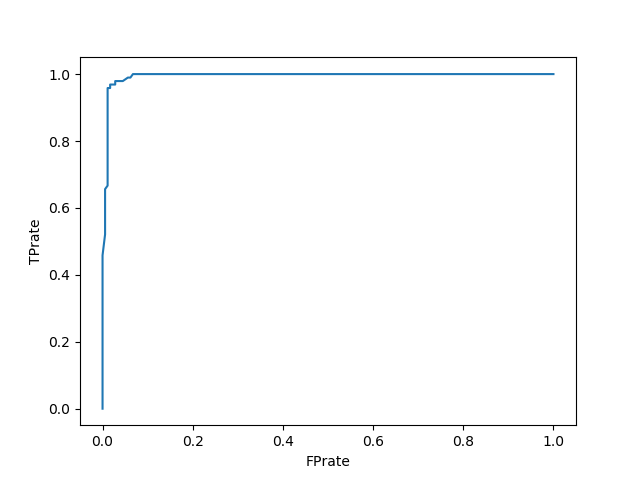
\includegraphics[scale=0.7]{ex5_roc}
\end{center}
The area under the curve is $0.995$ which is excellent.

\subsection{Part c}
The logistic classifier we obtained is slightly better than any of the bayesian model we previously computed:
it is the only one to reach more than $95\%$ in both precision and recall.
\\
One point we could argue with our previous modelisation is the use of Gaussian distributions for every feature
and projection along each direction.
\\
For example we can take a look at the distribution of values for the «Micoses» feature we used for each class:
\begin{center}
   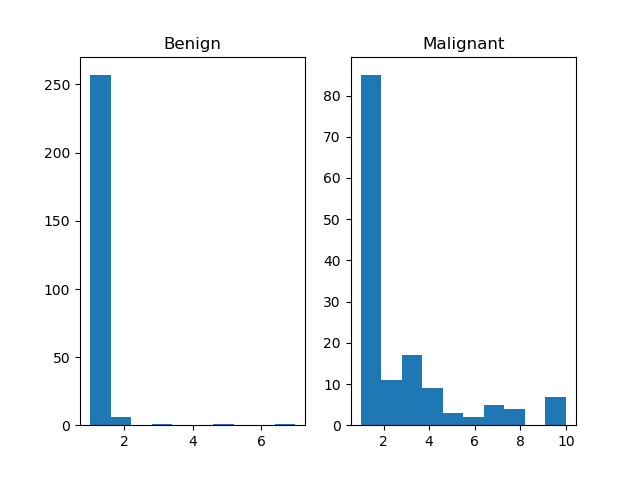
\includegraphics[scale=0.7]{micoses} 
\end{center}
The distribution for the benign data could be approximated to Gaussian with very low variance but
for the malignant tumors, the histogram is clearly not symmetric.
\\
We can draw over the plot the approximation we made by supposing it was a Gaussian. After some normalization
to the hhistograms and plotting the Gaussian pdf:
\begin{center}
    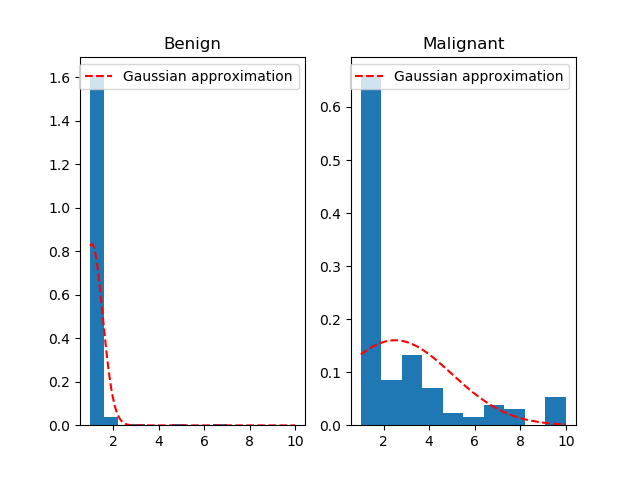
\includegraphics[scale=0.7]{micoses_gauss}
\end{center}
We clearly see that a normal distribution is not adapted.
\\
Moreover the values that our features take are always whole numbers between 1 and 10. Using a discrete
distribution would be more appropriate to modelize the data properly.
\end{document}
